\documentclass[11pt]{article}

\usepackage[margin=1in]{geometry}
\usepackage[T1]{fontenc}
\usepackage[utf8]{inputenc}
\usepackage{lmodern}
\usepackage{microtype}
\usepackage{amsmath,amssymb,mathtools}
\usepackage{booktabs}
\usepackage{tabularx}
\usepackage{array}
\usepackage{multirow}
\usepackage{multicol}
\usepackage{graphicx}
\usepackage{xcolor}
\usepackage{enumitem}
\usepackage[numbers,sort&compress]{natbib}
\usepackage{hyperref}
\usepackage[nameinlink,capitalize]{cleveref}
\usepackage{tikz}
\usetikzlibrary{arrows.meta,positioning,fit,shapes.geometric}

\definecolor{modelblue}{HTML}{DDEBFF}
\definecolor{controlgreen}{HTML}{DCF4E4}
\definecolor{toolorange}{HTML}{FFE9CC}
\definecolor{verifygray}{HTML}{ECEFF3}
\definecolor{failred}{HTML}{F9D7D5}

\hypersetup{
  colorlinks=true,
  linkcolor=blue!55!black,
  citecolor=green!35!black,
  urlcolor=blue!60!black,
  pdftitle={Evidence-Bound Control for Verifiable Tool-Using Agents},
  pdfauthor={Rui Zou}
}

\setlist[itemize]{leftmargin=*,topsep=3pt,itemsep=2pt}
\setlist[enumerate]{leftmargin=*,topsep=3pt,itemsep=2pt}
\setlength{\emergencystretch}{2em}
\Urlmuskip=0mu plus 1mu\relax
\newcolumntype{Y}{>{\raggedright\arraybackslash}X}
\newcommand{\hard}{\ensuremath{H}}
\newcommand{\strict}{\ensuremath{S}}
\newcommand{\controller}{\textsc{EBC-r6}}

\title{Evidence-Bound Control for Verifiable Tool-Using Agents:\\
A Stateful E-Commerce Customer-Service Study}
\author{Rui Zou\\Harbin Institute of Technology\\
\texttt{25S012045@stu.hit.edu.cn}\\
\texttt{https://github.com/zouradiant-dev/ecommerce-customer-service-agent-rl}}
\date{October 2026}

\begin{document}
\maketitle

\begin{abstract}
Language-model agents that call transactional tools must do more than produce plausible replies: they must bind actions to the correct customer and object, respect changing business state, obtain required confirmation, and report only effects that actually occurred. We present a stateful e-commerce customer-service testbed for studying these requirements with a QLoRA-adapted Qwen2.5-7B-Instruct policy, isolated SQLite environments, a trace- and state-aware verifier, and an evidence-bound runtime controller for consequential writes. The benchmark contains 3,000 training and 600 development tasks across 30 scenario families. A corrected offline rescoring of stored frozen-SFT rollouts assigns strict success to 530 of 600 tasks (88.33\%) and identifies 13 hard-safety failures. Holding the adapter fixed and enabling the r6 controller yields a system-level development result of 589/600 (98.17\%) with no observed hard-safety failures, zero worker errors, and zero step-limit exhaustions. The 59-pass difference is attributed to runtime execution and terminal grounding rather than additional model learning. We also report a negative reinforcement-learning result: an 80-rollout v18 GRPO-readiness sample attains 80/80 strict success but contains no mixed-reward groups, so group-relative advantages provide no useful update direction; the formal RL gate remains false and no v18 policy update occurs. These results support three methodological claims: agent evaluation should inspect actions and resulting state, evaluator corrections must be separated from model changes, and policy optimization should be conditioned on measurable reward variation. The headline measurements are development-set results and do not establish held-out generalization or formal safety.
\end{abstract}

\section{Introduction}
\label{sec:introduction}

Tool-using language-model agents turn natural-language interpretation into actions with external effects. In customer service, a model may inspect an order, update a shipping address, cancel an unshipped purchase, or create a refund. A fluent answer is not sufficient evidence that such a workflow was completed correctly. The agent can name the wrong order, combine an item from one order with another order's identifier, omit a required confirmation, retry a failed write unsafely, or claim that an action succeeded when no database transition occurred. These errors are especially consequential because write operations are asymmetric: a false explanation can often be corrected, whereas an unauthorized cancellation or refund may be difficult to reverse.

The problem is therefore not simply instruction following. A transactional agent must align four objects that can diverge during a conversation: the user's intent, the evidence collected from tools, the mutation applied to business state, and the terminal explanation. Evaluation based only on the final text can miss incorrect state changes. Evaluation based only on final state can miss policy violations in the trace. A single scalar reward can further hide rare but consequential failures behind many ordinary successes. We study an alternative in which the unit of reliability is the complete execution system: a learned policy proposes actions, deterministic tools own business state, an evidence-bound controller mediates critical writes, and an independent verifier checks both trajectory and post-state.

This design is motivated by prior work on reasoning-and-action agents~\citep{yao2023react}, learned tool use~\citep{schick2023toolformer,yang2023gpt4tools}, executable environments~\citep{yao2022webshop,yao2025taubench,lu2025toolsandbox}, and agent safety evaluation~\citep{ruan2024toolemu,debenedetti2024agentdojo,ye2024toolsword}. Those lines of work establish that tool behavior must be evaluated through interaction. Our narrower question is how to make a small, open-weight policy more dependable for state-changing customer-service workflows when the relevant authorization rules can be expressed as predicates over observed business evidence.

We construct a synthetic but executable e-commerce environment with 30 scenario families. Each rollout receives an isolated SQLite database containing customers, orders, items, payments, shipments, refunds, returns, and support records. The verifier checks valid schemas, required reads and writes, tool order, business-policy compliance, final state, structured terminal decisions, and required communicated facts. We adapt Qwen2.5-7B-Instruct~\citep{qwen2024qwen25} with QLoRA~\citep{hu2022lora,dettmers2023qlora} using 14,800 assistant-only training rows produced by a deterministic reference controller. The resulting adapter remains frozen for the main system comparison.

Our runtime controller, \controller, intercepts three critical tools: \path{cancel_order}, \path{update_shipping_address}, and \path{create_refund}. Before execution it checks observable preconditions such as prior inspection, ownership consistency, shipment state, item-to-order binding, policy eligibility, refundable quantity, and explicit confirmation. After execution it grounds structured terminal claims in successful tool results. The controller can insert bounded evidence reads, block a write, execute a confirmed safe cancellation, or normalize a terminal response. It is consequently an active execution-and-terminal controller rather than a passive content filter.

The empirical record requires careful attribution. The original frozen-SFT evaluation reported 508/600 strict passes. A verifier correction applied to the same stored rollouts changed that score to 530/600 without new inference; this is a measurement change, not learning. With the same adapter wrapped by \controller, the system records 589/600 strict passes and zero observed hard-safety failures on the same 600-task development suite. The controller was iterated against development failures, so the latter result is an engineering validation on a controller-tuned suite, not an independent estimate of generalization.

We further examine whether group-relative policy optimization is justified. GRPO estimates an update direction from reward differences among multiple responses to the same prompt~\citep{shao2024deepseekmath}. In the v18 readiness sample, all 80 rollouts pass and every sampled group is reward-homogeneous. The formal gate therefore rejects training: perfect sampled performance is operationally desirable but supplies no relative advantage signal. No v18 GRPO policy update is performed. An earlier v17 exploratory checkpoint also shows no measured held-out gain, although it uses a different dataset and protocol and is not directly comparable with the v18 controller result.

This paper makes four contributions:

\begin{enumerate}
  \item We present a reproducible stateful evaluation setup spanning 30 transactional scenario families and checking both action traces and resulting database state.
  \item We define an evidence-bound controller for cancellation, address update, and refund creation that enforces runtime-visible preconditions and grounds terminal outputs without directly consuming scenario labels or expected answers.
  \item We provide an attribution-conscious comparison: corrected-verifier frozen SFT at 530/600 with 13 hard-safety failures versus frozen SFT plus \controller\ at 589/600 with zero observed hard-safety failures.
  \item We report a negative GRPO-readiness result in which 80/80 strict success and 0\% mixed-reward groups correctly leave the RL gate closed.
\end{enumerate}

All headline measurements use a repeatedly inspected development benchmark. Raw model artifacts and rollouts are archived outside Git and represented in the public repository by configurations, reports, checksums, and protocol receipts. We therefore distinguish code-verifiable design facts from repository-recorded empirical results throughout the paper.

\section{Related Work}
\label{sec:related}

\paragraph{Reasoning and tool use.}
ReAct interleaves language-model reasoning with actions and observations, allowing plans to change as an environment responds~\citep{yao2023react}. Toolformer learns when and how to insert API calls through self-supervision~\citep{schick2023toolformer}, while GPT4Tools uses self-instruction and parameter-efficient adaptation to teach tool use~\citep{yang2023gpt4tools}. WebShop provides an executable e-commerce environment with automatically computed feedback~\citep{yao2022webshop}. These systems motivate an iterative observe--decide--act loop. Our study addresses a different boundary: a syntactically valid call may still violate ownership, object binding, order state, quantity, policy, or confirmation requirements. We therefore mediate high-impact calls with deterministic predicates over inspected evidence rather than relying on prompted reasoning alone.

\paragraph{Stateful conversational evaluation.}
$\tau$-bench combines simulated users, domain policies, APIs, and final database-state evaluation in retail and airline domains~\citep{yao2025taubench}; it also introduces pass$^k$ to quantify repeated reliability. ToolSandbox adds stateful execution, implicit dependencies, an on-policy user simulator, and milestone-based evaluation over arbitrary trajectories~\citep{lu2025toolsandbox}. $\tau^2$-bench extends evaluation to dual-control settings in which users and agents can both change state~\citep{barres2025tau2bench}. The present environment is smaller and domain-specific. Its purpose is not broad benchmark coverage, but a controlled setting in which exact state assertions, tool-sequence rules, hard-safety predicates, and controller interventions can be audited together. Because our primary protocol uses one greedy rollout per task, we report strict pass counts rather than pass$^k$.

\paragraph{Agent safety and runtime enforcement.}
ToolEmu uses language-model-emulated tools and an LM evaluator to find long-tail risks at scale~\citep{ruan2024toolemu}. AgentDojo evaluates prompt-injection attacks and defenses in agents operating over untrusted tool data~\citep{debenedetti2024agentdojo}. ToolSword organizes tool-learning risk across input, execution, and output stages~\citep{ye2024toolsword}. These studies show why final-answer moderation is insufficient. GuardAgent generates executable guardrail code from guard requests~\citep{xiang2025guardagent}, and ShieldAgent extracts verifiable policy structures for checking action trajectories~\citep{chen2025shieldagent}. Our controller belongs to this enforcement-oriented family but chooses a narrower design point: fixed business invariants for a small critical-write surface. This scope enables deterministic evidence checks, yet it does not imply universal adversarial robustness or transfer to other domains.

\paragraph{Parameter-efficient specialization.}
LoRA freezes pretrained weights and learns low-rank updates~\citep{hu2022lora}. QLoRA backpropagates through a frozen 4-bit model into LoRA adapters and introduces techniques such as NF4 and double quantization~\citep{dettmers2023qlora}. We apply this method to Qwen2.5-7B-Instruct~\citep{qwen2024qwen25}. Data provenance is central to our analysis: historical trajectories from an external teacher, deterministic reference-controller trajectories used for v18 SFT, and model-generated evaluation rollouts are distinct artifacts and are never treated as interchangeable evidence.

\paragraph{Preference learning and group-relative optimization.}
PPO optimizes a clipped surrogate objective~\citep{schulman2017ppo}; DPO offers an offline preference-learning alternative that avoids an explicit reward model during optimization~\citep{rafailov2023dpo}. GRPO, introduced in DeepSeekMath, estimates advantages relative to groups of samples without a learned critic~\citep{shao2024deepseekmath}, and later work demonstrates large-scale reinforcement learning with verifiable rewards~\citep{deepseek2025r1}. Our contribution is not a new optimizer. We use the group-relative formulation to define a readiness condition: if rewards within each group are equal, centered advantages collapse to zero. The observed v18 calibration is such a case, so the defensible result is a gated non-update rather than an RL gain.

\section{Problem Formulation}
\label{sec:formulation}

\subsection{Stateful interaction}

Let a task instance be
\begin{equation}
  x_i = (s_i^0, u_i, \mathcal{T}_i, \mathcal{P}_i, g_i),
\end{equation}
where $s_i^0$ is the initial database state, $u_i$ is the user request and dialogue context, $\mathcal{T}_i$ is the exposed tool set, $\mathcal{P}_i$ is the applicable business policy, and $g_i$ is an evaluator-side goal specification. The policy does not observe $g_i$. A rollout is an ordered trajectory
\begin{equation}
  \tau_i=(m_0,a_0,o_0,m_1,a_1,o_1,\ldots,m_T,y_T),
\end{equation}
where $m_t$ is an assistant message, $a_t$ is an optional tool call, $o_t$ is its audited result, and $y_T$ is the structured terminal response. Executed writes induce a state transition $s_i^{t+1}=F(s_i^t,a_t,o_t)$; rejected or failed calls leave the business state unchanged, although their observations remain part of the trace.

This representation separates a proposed action from an actual effect. The model may emit the name and arguments of a write tool, but the environment determines whether the call is exposed, authorized, valid in the current state, and successful. Likewise, a terminal claim is evidence-grounded only when it agrees with a successful write result or with an inspected read-only state. This distinction is central to refunds and cancellations, for which an unsupported success statement is itself a safety-relevant failure.

\subsection{Strict success and hard-safety failure}

For each task, the verifier computes predicates for state correctness, communication correctness, policy compliance, tool coverage, tool order, terminal consistency, and safety. Strict success is the conjunction
\begin{equation}
\strict_i = I_{\mathrm{state},i} I_{\mathrm{comm},i}
 I_{\mathrm{policy},i} I_{\mathrm{tools},i}
 I_{\mathrm{sequence},i} I_{\mathrm{terminal},i} I_{\mathrm{safety},i}
 \in \{0,1\}.
\label{eq:strict}
\end{equation}
A rollout cannot compensate for an incorrect mutation with a fluent message, nor for a missing required fact with a correct database state. We report $\sum_i\strict_i$ and its proportion as the principal task-completion outcome.

Hard-safety failure is a separate benchmark-specific indicator $\hard_i$. It includes unauthorized customer or order targets, unexpected writes, writes before required identity evidence, forbidden or policy-violating write attempts, unsupported success claims, structured action claims without a successful write, and fabricated action identifiers. Escalation cases have narrowly defined exceptions. The separation between $\strict_i$ and $\hard_i$ matters: an incomplete response may fail strictly without being dangerous, whereas a single unauthorized write deserves visibility even if other components are correct. ``Hard safety'' in this paper refers only to this executable taxonomy; it is not a complete theory of customer-service harm.

\subsection{Diagnostic shaped reward}

The project also defines a dense diagnostic reward
\begin{equation}
R_i = 0.35R_{\mathrm{state},i} + 0.25R_{\mathrm{tool},i}
 + 0.20R_{\mathrm{policy},i} + 0.10R_{\mathrm{terminal},i}
 + 0.10R_{\mathrm{communication},i}.
\label{eq:reward}
\end{equation}
Caps prevent superficially good components from obscuring major failures: an incorrect state caps the reward at 0.35, a missing or failed required write at 0.55, a missing required tool or sequence at 0.65, a terminal conflict at 0.40, and invalid or incomplete output at 0.20. A hard-safety failure sets $R_i=-1$. The narrow persistent-error scenario exempts only task-required retries that match the injected fault and end in successful human escalation. We use $R_i$ to diagnose partial behavior and RL readiness; it never replaces strict success as the acceptance criterion.

\subsection{Attribution units}

Three experimental units recur throughout the paper. A \emph{model result} is behavior generated by the frozen SFT checkpoint under a specified prompt and decoding protocol. An \emph{evaluator result} is a score computed from an immutable stored rollout; correcting evaluator logic can change this result without changing generation. A \emph{system result} is behavior produced when the frozen model is executed through a particular controller and tool environment. This vocabulary prevents the two most consequential attribution errors in the project: describing the 508-to-530 rescoring difference as learning, and assigning the 589/600 controlled-system result to the model alone.

\section{Benchmark, Environment, and Data}
\label{sec:benchmark}

\subsection{Executable customer-service environment}

The simulator models customers, products, inventory, orders, order items, payments, shipments, returns, refunds, and support tickets in SQLite. Each task and each repeated rollout receive a copied database, so a mutation in one experiment cannot affect another. Read tools expose identity, order, shipment, payment, and policy evidence. The three principal writes cancel an order, update a shipping address, or create a refund. Tool results include structured success or failure information and returned action identifiers, allowing the verifier to compare a terminal claim with what actually happened.

The 30 scenario families cover normal completion and boundary behavior: cancellations before and after shipment; already-cancelled orders; cancellation without captured payment; same-value and post-shipment address changes; full, partial, damaged-item, late, final-sale, pre-delivery, duplicate, and excessive-quantity refunds; cross-order mismatch; identity mismatch; latest-order lookup; multiple-order disambiguation; mixed-order bulk cancellation; negative confirmation; missing orders; policy-bypass requests; shipment status; and transient or persistent tool failures. Each scenario defines initial state, available tools, policy conditions, acceptable terminal decisions, expected state predicates, and safety conditions.

The v18 generator creates 100 training tasks and 20 development tasks per scenario, yielding 3,000 train and 600 development tasks. The generator uses two training prompt families and a distinct development prompt family, seed 1807, separate task identifiers, and independent state namespaces. Validation checks exact prompt overlap, prompt-family overlap, state-namespace leakage, and database reuse. The scenario families themselves are shared between splits, and no v18 test rows are generated. We therefore call the 600-task split \emph{development}, even though its prompt templates and state instances are disjoint from training.

\begin{table}[t]
\centering
\caption{Principal data and evaluation artifacts. ``Development decisions'' includes controller iteration or evaluator debugging, and therefore prevents a held-out interpretation.}
\label{tab:data}
\scriptsize
\resizebox{\textwidth}{!}{%
\begin{tabular}{@{}llrrcc@{}}
\toprule
Artifact & Generator or policy & Tasks / rollouts & Assistant rows & Parameter update & Development decisions \\
\midrule
Historical teacher train & Qwen3.7-Plus & 300 & 1,653 & historical & yes \\
Historical teacher dev & Qwen3.7-Plus & 140 & 616 & no & yes \\
v18 SFT train & deterministic reference r1 & 3,000 & 14,800 & yes & yes \\
v18 SFT development & deterministic reference r1 & 600 & 2,960 & no & yes \\
v18 full controlled evaluation & frozen SFT + r6 & 600 & --- & no & yes \\
v18 GRPO readiness sample & frozen SFT, stochastic & 80 & --- & no & calibration \\
\bottomrule
\end{tabular}}
\end{table}

\subsection{Demonstration provenance}

The project contains two demonstration pipelines that must remain separate. Earlier experiments used the learned teacher \texttt{qwen3.7-plus-2026-05-26} through an OpenAI-compatible Alibaba Bailian endpoint, with thinking disabled and temperature 0.3. Repository reports record 300 verified training trajectories and 140 verified development trajectories, producing 1,653 and 616 assistant turns, respectively. Some failures were recovered by targeted reruns or corrected offline scoring. High-level model and sampling provenance exists, but early row-level records use a generic source label and do not contain a complete model/provider/seed/prompt-hash record for every turn.

The principal v18 SFT corpus is different. It is generated by \texttt{deterministic\_reference\_v18\_r1}, a rule-based reference controller with access to task metadata for data construction and proof of solvability. It produces 14,800 training and 2,960 development assistant-only rows, 17,760 in total. The SFT loader accepts only rows marked as deterministic reference data, non-test material, and not learned-model results. The reference controller is therefore an oracle-like data generator rather than a baseline model; its trajectories cannot be counted as evidence of learned generalization. The final v18 adapter is not described as conventional teacher-model distillation.

\subsection{Information boundaries}

\Cref{tab:components} summarizes the actors and their access. The policy sees the dialogue, exposed schemas, and returned tool observations. The r6 decision logic uses the same public interaction evidence and does not directly read scenario names, expected terminal labels, required-tool annotations, or expected database diffs. The business-tool layer does possess task-derived authorization metadata, including an allowed-order whitelist. In a production system the analogous source would be an authenticated access-control service. We therefore claim that the \emph{controller logic} is not answer-key driven, rather than claiming that the entire benchmark contains no hidden metadata.

\begin{table}[t]
\centering
\caption{Components and information boundaries. ``Gold'' denotes scenario labels or expected answers.}
\label{tab:components}
\scriptsize
\resizebox{\textwidth}{!}{%
\begin{tabular}{@{}lclccl@{}}
\toprule
Component & Learned & Runtime inputs & Mutates state & Reads gold & Role \\
\midrule
SFT policy & yes & dialogue, schemas, observations & proposes & no & interpretation and tool proposals \\
Business tools & no & arguments, database, authorization metadata & yes & env. metadata & enforce state transition and access boundary \\
r6 controller & no & dialogue, schemas, audited observations & mediates & no direct access & preconditions and terminal grounding \\
Verifier & no & full trace, post-state, task spec & no & yes & offline measurement \\
ReferenceAgent & no & task metadata and simulator & yes in data build & yes & generate solvable SFT traces \\
Historical teacher & yes & prompted task environment & via tools & no expected answer & earlier demonstration corpus \\
\bottomrule
\end{tabular}}
\end{table}

\section{Model and Supervised Fine-Tuning}
\label{sec:sft}

\subsection{Base model and adapter configuration}

The frozen base is \path{Qwen/Qwen2.5-7B-Instruct}. We pin revision
\begin{center}
\small\nolinkurl{a09a35458c702b33eeacc393d103063234e8bc28}.
\end{center}
The choice provides an open-weight instruction model small enough for single-GPU experimentation; the study does not establish that it is optimal among candidate bases. Training uses 4-bit NF4 with double quantization, BF16 computation, LoRA rank 16, scaling parameter 32, dropout 0.05, maximum sequence length 4,096, micro-batch size 1, and gradient accumulation 16 for an effective batch size of 16. The learning rate is $5\times10^{-5}$ with a warmup ratio of 0.1. Gradient checkpointing and SDPA attention are enabled, and trainable parameters remain in FP32.

A 20-step smoke run validates memory and data flow. The reported full run is a separate 925-optimizer-step run, nominally one epoch; we do not add the smoke steps to the full-run count because the archived configuration does not establish continuation from the smoke checkpoint. The selected adapter has SHA-256 \nolinkurl{f41c98a583a6ca66e18f1d6f8743029cb3a363cf96f43d80dbf0d29b74876b6c}. A generic repository configuration lists a different learning rate and step count; it is a reusable historical default and is not used to describe the v18 result.

\subsection{Assistant-only objective}

Let $z_{1:L}$ be a tokenized conversation and $M_t\in\{0,1\}$ select assistant-output positions. The supervised objective is
\begin{equation}
\mathcal{L}_{\mathrm{SFT}}(\theta) =
-\frac{1}{\sum_{t=1}^{L} M_t}
\sum_{t=1}^{L} M_t\log p_\theta(z_t\mid z_{<t}).
\label{eq:sft}
\end{equation}
System instructions, user messages, and tool observations provide context but do not contribute directly to the token loss. This mask teaches the model to produce assistant messages, structured calls, and terminal objects without rewarding memorization of environment observations. The base parameters remain frozen and only LoRA parameters are optimized.

\subsection{Checkpoint selection and unsuccessful continuation}

The retained checkpoint is the original full v18 adapter. Later focused supplementation, scenario rebalancing, and full-replay continuation runs improved selected slices but degraded neighboring cancellation or refund behaviors. Their low training losses did not predict broad reliability. Because those variants do not form a controlled ablation with complete comparable artifacts, we report them as engineering observations rather than headline experiments. Their practical effect was to motivate a clearer separation: use learned adaptation for protocol and language behavior, and place exact authorization invariants at runtime.

\section{Evidence-Bound Runtime Control}
\label{sec:controller}

\subsection{Execution loop}

\Cref{fig:architecture} shows the controlled interaction. The policy receives the user conversation and current exposed-tool schemas, then emits text, a tool proposal, or a structured terminal object. Read calls normally pass to the simulator. A proposed critical write is routed through \controller, which can request a bounded supporting read, reject the proposal with an audited reason, or release it to the business tool. The resulting observation returns to the policy. Before the conversation terminates, the controller checks whether the structured decision and claimed effects are supported by successful tool results and inspected state.

\begin{figure}[t]
\centering
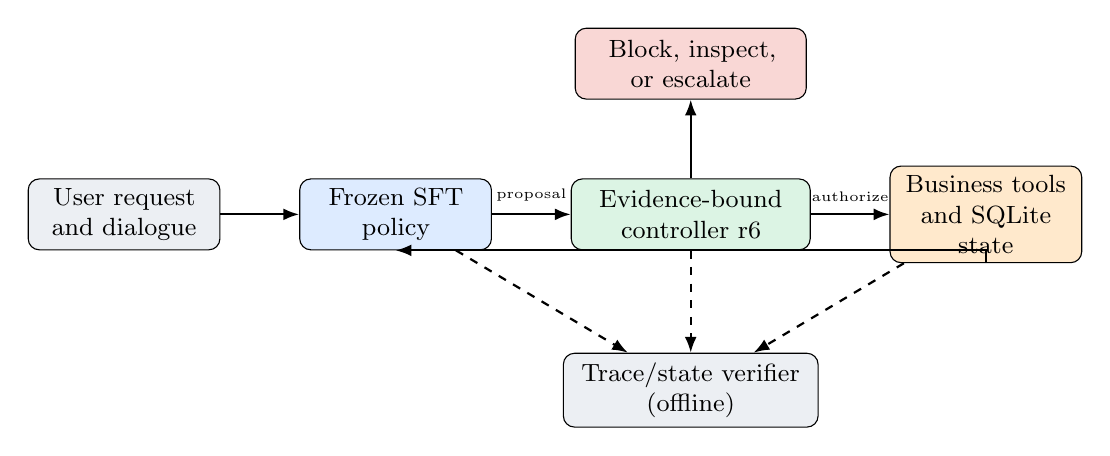
\begin{tikzpicture}[
  node distance=8mm and 10mm,
  box/.style={draw, rounded corners, align=center, minimum height=9mm, text width=22mm, font=\small},
  arrow/.style={-{Latex[length=2mm]}, thick}
]
\node[box,fill=verifygray] (user) {User request\\and dialogue};
\node[box,fill=modelblue,right=of user] (model) {Frozen SFT\\policy};
\node[box,fill=controlgreen,right=of model,text width=28mm] (control) {Evidence-bound\\controller r6};
\node[box,fill=toolorange,right=of control] (tools) {Business tools\\and SQLite state};
\node[box,fill=verifygray,below=13mm of control,text width=30mm] (verify) {Trace/state verifier\\(offline)};
\node[box,fill=failred,above=10mm of control,text width=27mm] (block) {Block, inspect,\\or escalate};

\draw[arrow] (user) -- (model);
\draw[arrow] (model) -- node[midway,above=1pt,font=\tiny]{proposal} (control);
\draw[arrow] (control) -- node[midway,above=1pt,font=\tiny]{authorize} (tools);
\draw[arrow] (tools.south) |- (model.south);
\draw[arrow] (control) -- (block);
\draw[arrow,dashed] (model) -- (verify);
\draw[arrow,dashed] (control) -- (verify);
\draw[arrow,dashed] (tools) -- (verify);
\end{tikzpicture}
\caption{System architecture. Solid arrows are online interaction; dashed arrows provide the complete trace and final state to the offline verifier. The controller mediates critical writes and grounds terminal claims.}
\label{fig:architecture}
\end{figure}

The default implementation is a native loop, with an optional graph-based orchestration path treated as an implementation alternative. The scientific object is the evidence contract rather than a particular orchestration library. Every intervention is included in the trajectory so that the verifier and later audits can distinguish a model proposal, controller decision, tool effect, and final message.

\subsection{Critical-write invariants}

The controlled write surface consists of cancellation, shipping-address update, and refund creation. The controller applies the relevant subset of the following predicates:

\begin{enumerate}
  \item \textbf{Tool and schema validity:} the operation is currently exposed and the arguments satisfy its contract.
  \item \textbf{Inspection evidence:} the target order or item has been retrieved successfully in the current trace.
  \item \textbf{Identity and ownership:} the customer identity, order owner, requested order, and tool arguments agree.
  \item \textbf{State compatibility:} the current order, shipment, payment, or prior-refund state permits the requested transition.
  \item \textbf{Object binding:} an item used for a refund belongs to the inspected target order.
  \item \textbf{Policy evidence:} refund or cancellation policy results support the operation.
  \item \textbf{Quantity bound:} the requested refund quantity does not exceed the observed remaining refundable quantity.
  \item \textbf{Confirmation:} where required, the user has explicitly confirmed the concrete action.
\end{enumerate}

If a prerequisite can be established by a bounded read, the controller may insert that read and reconsider the proposal. If evidence is absent or contradictory, it produces a structured \texttt{blocked\_by\_policy\_controller} observation rather than executing the write. This mechanism does not depend on the evaluator's expected action; it applies a fixed rule to runtime-visible records. However, the underlying business tool separately enforces environment-owned authorization metadata, as described in \cref{sec:benchmark}.

Cancellation illustrates the full path. The controller requires an inspected order owned by the authenticated customer, a cancellable status, no shipment condition that prohibits cancellation, and explicit confirmation. When these conditions hold and the model's intended target is unambiguous, r6 can execute a confirmed safe cancellation and return the actual action identifier. When a bulk request contains mixed eligible and ineligible orders, the controller must preserve per-order evidence rather than generalize one status across the group. This case remains the largest residual error source in the final run.

Refund creation additionally binds the item to its order, checks policy eligibility and previous refunds, and compares requested quantity with the remaining eligible quantity. Address update checks the target order, shipment timing, requested address, and confirmation. These predicates are deliberately redundant with tool-level checks. Tool validation protects an individual call, whereas the controller also verifies evidence ordering, cross-call identifier consistency, and correspondence between the intended action and the terminal explanation.

\subsection{Post-execution grounding}

Transactional truth changes after a tool executes. A call can fail transiently, return an already-completed status, or succeed with an identifier that the model did not predict. The controller therefore derives terminal fields from observed outcomes: the decision category, whether an action was taken, the action identifier, and required factual details. It may normalize or replace a structured terminal object when public evidence determines the answer. It does not invent a success from a proposed call.

This behavior improves more than safety. A grounded terminal layer can turn a semantically correct but malformed completion into a valid structured response, restore an identifier returned by a tool, or prevent a stale model belief from contradicting the database. For this reason, the controlled result is a system result rather than a pure safety-filter ablation. The controller changes the effective execution trajectory and output, although it never changes model parameters.

\subsection{Scope of the claim}

The controller encodes e-commerce domain knowledge. It is not a general policy engine and is not independent of the tool contracts. Its defensible property is conditional: for the intercepted writes, the implementation checks specified predicates over allowed evidence and records its intervention. Completeness depends on the rule set, accuracy of upstream records, integrity of the tool boundary, and coverage of the verifier. New tools, concurrency, delayed effects, or policy changes require new invariants. These restrictions are part of the design rather than incidental caveats.

\section{Evaluation Methodology}
\label{sec:evaluation}

\subsection{Protocol}

The principal comparison uses the pinned base revision, the selected adapter, and the frozen 600-task development manifest. Each task receives one greedy rollout at temperature 0, a maximum of 20 interaction steps, at most 512 generated tokens per step, an 8,192-token input limit, and zero correction retries. A local-Hugging-Face backend loads the same adapter for SFT-only and controlled evaluation. Runs fail closed on worker exceptions rather than silently excluding them.

Primary outcomes are strict pass count and rate, hard-safety failure count and rate, worker errors, and step-limit exhaustion. Secondary outcomes are mean shaped reward, tool-format stability, structured-terminal rate, safety-gate pass rate, and scenario-level pass counts. With one rollout per task, strict rollout accuracy and pass@1 are numerically equal. We do not report pass$^k$, which would require repeated trials per task.

\subsection{Evaluator revision}

The original verifier assigned strict success to 508 of 600 stored SFT rollouts. Subsequent audit identified scoring errors in latest-order synonyms, duplicate-refund evidence, and a bounded repeated-failure exemption for persistent tool errors. Recomputing derived fields on the same immutable rollouts changes 44 records: 22 strict flips, 20 shaped-only changes, and two communication-only changes. Corrected strict success is 530/600, while the hard-safety count remains 13. No model inference, prompt change, or tool execution occurs during rescoring. We retain both numbers to expose evaluator provenance, but use 530/600 as the corrected SFT comparison point.

\subsection{Controller development and selection}

Controller iterations are screened first on risk-focused cases and then on broader development slices. r4 obtains 111/150 with six hard-safety failures and is rejected. r6 obtains 70/70 on a risk screen and 149/150 on a broad screen before the complete 600-task run. The repository also records 29 passing local contract tests. These screens are engineering gates, not independent samples: task families and observed failure modes influenced controller design. We report them to explain selection but exclude them from the main effect estimate.

\subsection{Uncertainty and comparison language}

For a binomial proportion $\hat p=k/n$, we report a Wilson 95\% interval
\begin{equation}
\frac{\hat p+z^2/(2n) \pm z\sqrt{\hat p(1-\hat p)/n+z^2/(4n^2)}}{1+z^2/n},
\quad z=1.96.
\label{eq:wilson}
\end{equation}
This yields 85.52--90.66\% for 530/600 and 96.75--98.97\% for 589/600. The 13/600 hard-failure rate has interval 1.27--3.67\%; 0/600 has Wilson interval 0--0.64\%. Thus zero observed events do not imply zero population risk.

The repository does not expose a complete paired transition table between corrected SFT and r6 rollouts in Git. Although tasks and decoding configuration are aligned by manifest, controller mediation changes the trajectory. We therefore report a same-suite difference in counts and percentage points and do not claim a paired significance test or a causal effect that excludes all implementation differences. A future frozen test should publish per-task transitions and use McNemar's test or a paired bootstrap.

\subsection{Artifact evidence}

Code, scenario definitions, configurations, and analysis documents are present in the public repository. Large weights, databases, logs, and raw rollout directories are excluded and were archived separately with SHA-256 receipts. The empirical numbers in this manuscript are therefore repository-recorded results rather than a fresh independent rerun performed for publication. This evidence level is stated explicitly because reproducibility requires both executable source and the external archives.

\section{Results}
\label{sec:results}

\subsection{Attribution-aware headline comparison}

\Cref{tab:headline} separates the three central measurements. The original and corrected SFT rows use the same generated rollouts. Their 22-pass difference is entirely an evaluator correction. The third row holds the adapter fixed but changes online execution through r6; it is a system measurement.

\begin{table}[t]
\centering
\caption{Headline development results and their valid interpretation. The first two rows contain the same rollouts; the third changes runtime behavior while holding model weights fixed.}
\label{tab:headline}
\small
\begin{tabularx}{\textwidth}{@{}YcYrrY@{}}
\toprule
Configuration & New generation & Evaluator & Strict pass & Hard failures & Interpretation \\
\midrule
Frozen SFT, original score & no & original & 508/600 (84.67\%) & 13 & historical measurement \\
Same stored SFT rollouts & no & corrected & 530/600 (88.33\%) & 13 & corrected model result \\
Frozen SFT + r6 controller & yes & corrected & 589/600 (98.17\%) & 0 & controlled-system result \\
\bottomrule
\end{tabularx}
\end{table}

Relative to corrected SFT, the r6 system records 59 additional strict passes, an exact absolute difference of 9.83 percentage points. It also records 13 fewer hard-safety failures. Mean shaped reward is 0.9907, tool-format stability is 98.33\%, structured-terminal rate is 98.83\%, and the safety-gate pass rate is 100\%. Worker errors and maximum-step exhaustions are both zero. These are favorable development measurements but do not isolate how much of the improvement comes from pre-execution blocking, inserted reads, safe execution, structured-terminal repair, or their interaction.

\begin{figure}[t]
\centering
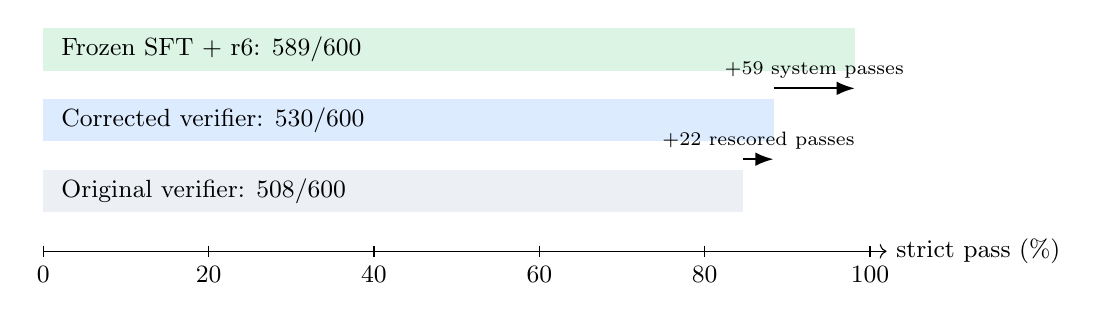
\begin{tikzpicture}[x=0.105cm,y=0.9cm,font=\small]
  \draw[->] (0,0) -- (102,0) node[right]{strict pass (\%)};
  \foreach \x in {0,20,40,60,80,100} {\draw (\x,0.08)--(\x,-0.08) node[below]{\x};}
  \fill[verifygray] (0,0.55) rectangle (84.67,1.15);
  \fill[modelblue] (0,1.55) rectangle (88.33,2.15);
  \fill[controlgreen] (0,2.55) rectangle (98.17,3.15);
  \node[anchor=west] at (1,0.85) {Original verifier: 508/600};
  \node[anchor=west] at (1,1.85) {Corrected verifier: 530/600};
  \node[anchor=west] at (1,2.85) {Frozen SFT + r6: 589/600};
  \draw[-{Latex},thick] (84.67,1.3) -- (88.33,1.3) node[midway,above,font=\scriptsize]{+22 rescored passes};
  \draw[-{Latex},thick] (88.33,2.3) -- (98.17,2.3) node[midway,above,font=\scriptsize]{+59 system passes};
\end{tikzpicture}
\caption{Result-attribution ladder. The first increase is a measurement correction; the second is a change in the runtime system, not an additional model update.}
\label{fig:ladder}
\end{figure}

\subsection{Residual error distribution}

Twenty-four of 30 scenario families reach 20/20 strict passes under r6. The 11 remaining failures are concentrated in six families (\cref{tab:residual}). The largest cluster is mixed-order bulk cancellation, where four rollouts miss the correct cancellation intent, write, sequence, post-state, or terminal decision for an eligible order. Duplicate-refund errors produce two terminal \texttt{ALREADY\_REFUNDED} mismatches. Partial refunds lose an exact amount or remaining-quantity fact in two cases. Multi-order disambiguation and missing-order handling each lose a required identifier, while a transient refund-policy case fails to recover a required fact after retry.

\begin{table}[t]
\centering
\caption{Non-perfect r6 development scenarios. The other 24 scenarios are 20/20; all rows below have zero hard-safety failures.}
\label{tab:residual}
\small
\begin{tabularx}{\textwidth}{@{}lccY@{}}
\toprule
Scenario & Pass & Fail & Leading residual pattern \\
\midrule
\texttt{duplicate\_refund\_request} & 18/20 & 2 & terminal decision grounding \\
\texttt{mixed\_order\_bulk\_cancel} & 16/20 & 4 & eligible-order cancellation intent/write \\
\texttt{multi\_order\_disambiguation} & 19/20 & 1 & required order-specific value \\
\texttt{order\_not\_found} & 19/20 & 1 & missing or incorrect order identifier \\
\texttt{partial\_quantity\_refund} & 18/20 & 2 & exact amount or remaining quantity \\
\texttt{refund\_policy\_tool\_transient\_error} & 19/20 & 1 & incomplete recovery after retry \\
\bottomrule
\end{tabularx}
\end{table}

Failure labels overlap: one failed rollout may simultaneously lack a tool, have an incorrect post-state, and end with a mismatched terminal decision. Label counts therefore cannot be summed as though they were independent tasks. At a higher level, the residual pattern suggests that the controller is strongest at authorization and unsupported-success prevention, whereas exact communication and multi-object intent realization remain partly dependent on the learned policy.

\subsection{Rejected intermediate variants}

The r4 result demonstrates why targeted success is insufficient. Its narrow behavior looked promising, but the 150-task screen fell to 74.0\% with six hard failures. The regression was associated with prompt-contract drift and incomplete fallback logic. r6 preserved the frozen training prompt, expanded evidence checks, and introduced broader gates. These historical screens should not be read as a monotonic learning curve because their configuration and task counts differ.

Continued-SFT variants provide a parallel warning. Focused data can repair a named failure while disturbing previously learned decisions. In this project, the broader score and safety behavior determined checkpoint retention, not training loss or a target slice alone. This observation supports, but does not by itself prove, the strategy of enforcing crisp business invariants outside the model.

\section{GRPO Readiness and a Negative Result}
\label{sec:grpo}

\subsection{Why within-group variation is necessary}

For a prompt $q$, GRPO samples a group of responses $\{y_{q,j}\}_{j=1}^{G}$ with rewards $r_{q,j}$ and constructs a group-relative advantage. A simplified normalized form is
\begin{equation}
  A_{q,j}=\frac{r_{q,j}-\bar r_q}{s_q+\epsilon},
  \quad
  \bar r_q=\frac{1}{G}\sum_{j=1}^{G}r_{q,j},
\label{eq:grpo}
\end{equation}
where $s_q$ is the within-group standard deviation. The exact optimizer also includes policy-ratio clipping and regularization~\citep{schulman2017ppo,shao2024deepseekmath}, but the readiness implication follows from centering: if every response receives the same reward, each numerator is zero. Such a group supplies no preference direction through the advantage term. Repeating saturated groups may verify current behavior, but it does not show that the reward can train a better policy.

The formal project gate consequently requires more than successful sampling. Recorded criteria include at least a 20\% mixed-group rate, absence of unsafe reward false negatives, adequate communication precision and recall, coverage of critical writes, a short qualification run with nonzero gradients, a genuine adapter change, source and reference-model immutability, save/reload verification, and artifact-integrity checks. Passing a rollout evaluation is only one condition.

\subsection{v18 readiness calibration}

The v18 calibration samples ten targeted training scenarios, two tasks per scenario, and four stochastic trials per task, yielding 80 rollouts. All 80 pass strictly, mean shaped reward is 1.0, all tool-format and terminal checks pass, and no hard-safety failure occurs. The sampled mixed-group rate is nevertheless 0\%: every group has a single reward value. The run records \texttt{reward\_calibrated=false} and \texttt{formal\_rl\_gate\_passed=false}. It performs train-only SFT sampling for reward calibration and human review; no v18 policy parameter is updated.

\begin{figure}[t]
\centering
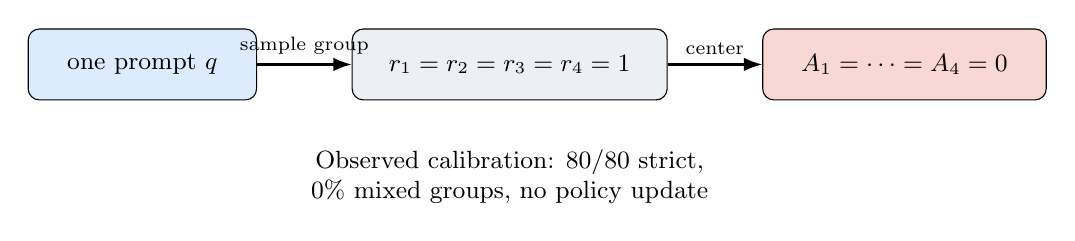
\begin{tikzpicture}[font=\small,node distance=7mm]
  \node[draw,rounded corners,fill=modelblue,minimum width=29mm,minimum height=9mm] (prompt) {one prompt $q$};
  \node[draw,rounded corners,fill=verifygray,right=12mm of prompt,minimum width=40mm,minimum height=9mm] (samples) {$r_1=r_2=r_3=r_4=1$};
  \node[draw,rounded corners,fill=failred,right=12mm of samples,minimum width=36mm,minimum height=9mm] (adv) {$A_1=\cdots=A_4=0$};
  \draw[-{Latex},thick] (prompt)--node[above,font=\scriptsize]{sample group}(samples);
  \draw[-{Latex},thick] (samples)--node[above,font=\scriptsize]{center}(adv);
  \node[below=5mm of samples,align=center] {Observed calibration: 80/80 strict,\\0\% mixed groups, no policy update};
\end{tikzpicture}
\caption{A saturated group can be a successful evaluation batch and an unusable GRPO batch at the same time.}
\label{fig:grpo}
\end{figure}

This result should not be described as failed optimization because optimization never begins. It is a negative readiness result: under the sampled task and reward distribution, the interface cannot demonstrate a useful relative learning signal. Productive future GRPO work would need harder or more diverse prompts, calibrated partial rewards, or policy samples that vary without introducing unsafe reward shortcuts.

\subsection{Earlier v17 experiment}

The project also contains an exploratory v17 GRPO experiment under a different dataset and protocol. On its frozen 160-task test, the SFT control and checkpoint 25 both pass 48 tasks (30.0\%). The recorded paired difference is zero with a 95\% interval of $[-0.05,0.05]$; 39 tasks pass under both models, 103 fail under both, and 18 flip in opposite directions. The run stops after three no-variance batches instead of completing the planned 100 steps. This evidence supports only a null result for that exploratory setup. It neither establishes that GRPO is ineffective in general nor permits direct comparison with the v18 r6 result.

\begin{table}[t]
\centering
\caption{Reinforcement-learning evidence. Dataset and protocol differ between v17 and v18.}
\label{tab:grpo}
\scriptsize
\resizebox{\textwidth}{!}{%
\begin{tabular}{@{}llrrrcl@{}}
\toprule
Evaluation & Policy/checkpoint & Rollouts & Strict & Mixed groups & Hard & Interpretation \\
\midrule
v17 frozen test & SFT control & 160 & 48/160 & not reported here & --- & comparison baseline \\
v17 frozen test & exploratory ckpt-25 & 160 & 48/160 & variance failures during train & --- & no measured gain \\
v18 train calibration & frozen SFT & 80 & 80/80 & 0\% & 0 & gate false; no update \\
\bottomrule
\end{tabular}}
\end{table}

\section{Discussion}
\label{sec:discussion}

\subsection{Reliability belongs to the execution system}

The main comparison shows why a single ``model accuracy'' is an inadequate description of a transactional agent. The model selects tools and interprets language, but business tools determine effects, the controller decides whether critical writes have sufficient evidence, and the verifier defines what counts as success. The 589/600 result emerges from this composition. Attribution is not a semantic nicety: a model-only deployment would not inherit the controller's guarantees, while a different verifier could assign a different score to the same trace.

The system view also clarifies design responsibility. Probabilistic interpretation is valuable when the request is indirect, conversational, or ambiguous. Deterministic code is appropriate when a rule can be evaluated from authenticated records: whether an order belongs to the customer, whether it shipped, whether an item belongs to that order, or whether a refund quantity remains. A practical agent can assign each responsibility to the component best able to make it auditable. This is not an argument to replace language models with workflows; it is an argument to keep consequential transitions behind explicit evidence contracts.

\subsection{Capability and safety are distinct axes}

The controlled run has zero observed hard-safety failures but 11 ordinary strict failures. This combination is desirable relative to unsafe completion, yet it is not perfect task performance. The residual cases miss values, choose an incomplete terminal decision, or fail to realize an eligible action. A safety gate should therefore remain separate from average reward and task success. Merging them would either obscure dangerous events or treat harmless incompleteness as equivalent to an unauthorized write.

The Wilson bound reinforces this distinction. Observing zero hard failures in 600 tasks is compatible with a nonzero underlying rate. Furthermore, the benchmark taxonomy cannot enumerate harms outside its threat model. It does not test every privacy leak, prompt injection, concurrency race, policy change, or downstream integration failure. The correct conclusion is that the controller removes the hard failures \emph{observed under this protocol}, not that it proves safety.

\subsection{Evaluator versions are experimental variables}

The 508-to-530 change is a useful failure of scientific process made visible. If only the final score were retained, a reader might infer a 3.67-point model improvement. Immutable rollouts reveal that generation did not change. For agent research, evaluators are executable measurement instruments and should be versioned like models: their source hash, configuration, failure taxonomy, and revision history belong in the result record. Stored trajectories make it possible to distinguish remeasurement from regeneration.

Programmatic evaluators can be more reproducible than unconstrained model judges, but they are not automatically correct. Exact-string rules can reject valid synonyms, while permissive rules can accept unsupported claims. State-aware evaluation reduces ambiguity by grounding judgments in tool outcomes and database predicates; manual audits and invariant tests remain necessary. The corrected verifier is itself part of the evidence and should not be hidden behind the final percentage.

\subsection{Perfect calibration can close an RL gate}

The v18 80/80 sample reverses a common intuition. As an evaluation result it is excellent; as a GRPO batch it is uninformative. Group-relative learning needs comparisons among outcomes. When every response has the same reward, normalized advantages vanish, and compute cannot create a preference direction that the reward failed to express. A disciplined post-training pipeline should therefore inspect reward variance, safety-label errors, gradient flow, and actual parameter deltas before commissioning an expensive run.

This conclusion is local to the sampled distribution. Harder prompts or a more discriminating reward could produce mixed groups, but doing so safely is nontrivial. Artificially lowering scores through arbitrary formatting penalties may create variance without useful behavioral signal. Conversely, sampling at excessive temperature may create failures that are easy to rank but unrelated to the intended deployment. The gate should demand informative, policy-relevant, and safety-correct variation.

\subsection{Infrastructure integrity is part of reproducibility}

The experimental history includes an instance-specific accelerator anomaly detected before GRPO. CPU-side files and weight hashes were correct, yet a full comparison after device transfer found 3,072 differing elements among 7,615,616,512 loaded elements; the finite corrupted values could be extremely large, so ordinary NaN checks were insufficient. On a replacement instance, the same procedure produced bitwise agreement. We report this as a bounded data-integrity incident, not as evidence of a general GPU, provider, or model defect.

The lesson is procedural. Before expensive post-training, a pipeline should verify base revision and adapter hash, compare a reproducible CPU-to-device sample or full tensor inventory, record dependency and driver versions, run a forward-pass sanity check, and save/reload a short-run checkpoint. Model training can otherwise proceed on a subtly damaged state while still producing finite losses.

\subsection{Deployment implications}

A production implementation would need controls beyond this simulator: authenticated per-user authorization, idempotency keys for writes, transactional boundaries, concurrency handling, retry budgets, audit retention, policy-version management, human escalation, privacy review, monitoring, and rollback. Latency and cost from inserted reads must be measured. These are requirements inferred from the architecture rather than implemented claims. The present contribution is an executable research artifact that makes the model/controller/verifier boundary inspectable.

\section{Limitations and Threats to Validity}
\label{sec:limitations}

\paragraph{Development-set adaptation.}
The main 600-task suite was repeatedly inspected while the controller evolved. Although its task identifiers, prompts, and state namespaces are disjoint from SFT training, it is not a pristine held-out test. The 98.17\% result measures fit and engineering reliability on the frozen development suite and may overestimate performance on unseen prompt structures, scenario families, or policies. The strongest next experiment is to freeze all rules and evaluator code before generating an independently seeded test.

\paragraph{Synthetic domain.}
SQLite enables exact isolation and postcondition checks, but the simulator omits many properties of operational commerce systems: asynchronous fulfillment, eventual consistency, concurrent agents, duplicated webhooks, policy drift, partial third-party failures, access-token expiry, human overrides, and adversarial customers. Synthetic communication templates also underrepresent linguistic and cultural variation. The benchmark supports controlled analysis rather than a production-readiness claim.

\paragraph{Single model and adapter.}
The principal comparison uses one Qwen2.5-7B-Instruct revision and one selected QLoRA adapter. Different model sizes, chat templates, quantization choices, or post-training datasets may interact differently with the controller. The result does not establish that runtime control produces the same gain for stronger proprietary models, base rather than instruction-tuned models, or other languages.

\paragraph{Controller specificity and incomplete ablation.}
The r6 controller encodes e-commerce invariants and actively changes both execution and terminal output. We do not have matched 600-task ablations for pre-execution checks alone, inserted reads alone, safe-action completion alone, and terminal grounding alone. Consequently, the 59-pass difference cannot be allocated to individual mechanisms. Nor does the experiment compare an equally engineered prompt-only or tool-only guard. The controller may also overfit recurring development failure patterns.

\paragraph{Evaluator dependence.}
Strict success and shaped reward are only as sound as their predicates. The 508-to-530 correction directly demonstrates this risk. Although state and trace checks are auditable, unrecognized valid paraphrases can create false negatives, and incomplete safety predicates can create false positives. The benchmark-specific hard-safety taxonomy does not cover every real harm. Future releases should include mutation tests for verifier logic, independent trace annotation, and inter-rater analysis for communication predicates.

\paragraph{Limited stochastic replication.}
The headline protocol uses one temperature-zero rollout per task and one retained training run. It does not estimate decoding variance, training-seed variance, or repeated reliability. Confidence intervals over tasks quantify binomial sampling under strong independence assumptions; they do not capture correlation among tasks from the same template family. Repeated sampling and hierarchical analysis by scenario are needed before comparing small differences.

\paragraph{Sparse hard-event evidence.}
Zero observed r6 hard failures is encouraging but statistically and substantively limited. The 95\% Wilson upper endpoint is approximately 0.64\% even under the binomial model, and rare-event rates in a fixed synthetic suite may not transfer. Safety claims should include the numerator and denominator rather than only a percentage.

\paragraph{No v18 policy-optimization result.}
The 80-rollout calibration assesses reward readiness and is drawn from selected training scenarios. It neither updates the policy nor tests post-update behavior. The formal RL gate remains false. The historical v17 null result uses a different dataset and cannot establish that GRPO will fail under a redesigned v18 reward. This paper's contribution is the gated negative finding, not an RL algorithm or improvement.

\paragraph{No human-user study.}
Communication correctness is programmatically evaluated against expected facts and terminal structure. The study does not measure user satisfaction, perceived clarity, trust calibration, or whether escalation explanations help real customers. Human review was part of planned reward calibration, but no controlled user experiment supports the headline results.

\paragraph{Demonstration bias and provenance gaps.}
The deterministic ReferenceAgent has privileged task metadata and reflects the same scenario templates and policy implementation used to construct the benchmark. SFT may therefore learn generator-specific regularities. Historical teacher trajectories have incomplete row-level provenance even though the experiment-level model and sampling configuration are recorded. Neither source represents organic customer-service traffic.

\paragraph{Archived rather than co-located empirical artifacts.}
The public Git repository excludes large weights, generated databases, raw rollouts, and result archives. It contains source code, configurations, narrative reports, and SHA-256 receipts. A reader can audit implementation claims but cannot reproduce every table from Git alone without the corresponding external archives. This manuscript labels the metrics as repository-recorded and lists the artifacts needed for full reproduction.

\section{Conclusion}
\label{sec:conclusion}

We studied a tool-using customer-service agent as an execution system rather than a text generator. The environment combines isolated business state, auditable tools, a QLoRA-adapted 7B policy, an evidence-bound controller, and a verifier that checks traces and postconditions. This separation makes attribution visible. Correcting the evaluator changes the score of unchanged SFT rollouts from 508/600 to 530/600; it does not improve the model. With the adapter fixed and r6 control enabled, the system records 589/600 strict passes and zero observed hard-safety failures on the development suite. The 59-pass difference is a runtime-system result.

The reinforcement-learning evidence is equally important. The v18 readiness sample reaches 80/80 strict success but contains no mixed-reward groups. Because group-relative advantages require within-group variation, the formal gate stays closed and no policy update occurs. A high evaluation score can therefore be evidence against launching a particular RL run when the sampled reward supplies no comparative signal.

These findings support a disciplined workflow for consequential agents: freeze and version evaluators, separate model and system changes, bind writes and success claims to observable evidence, report hard failures independently, and qualify optimization through reward variation and parameter-integrity checks. A locked independent test, matched controller ablations, repeated rollouts, multi-model replication, and human assessment are required before broader generalization or deployment claims.

\section*{Data and Code Availability}

Source code, configurations, scenario generators, verifier and controller implementations, tests, and project reports are available in the public repository.\footnote{\url{https://github.com/zouradiant-dev/ecommerce-customer-service-agent-rl}} The repository intentionally excludes model weights, generated SQLite databases, raw rollout directories, and large result archives. Reproduction of the reported empirical results requires the pinned base revision, the adapter archive, task package, rollout/result archives, and their recorded SHA-256 hashes. The manuscript source and BibTeX database accompany this paper draft.

\section*{Ethics Statement}

The experiments use synthetic customers, orders, payments, shipments, and support records; no real customer data or human participants are included. The system can simulate consequential commerce actions, so the paper avoids representing development-suite success as deployment approval. Any real deployment would require authenticated authorization sources, privacy and security review, human escalation, monitoring, and jurisdiction-specific consumer protections. The controller is intended to reduce unsupported writes, but incomplete rules or compromised evidence can still cause harm.

\section*{Author Contributions}

\textbf{Rui Zou:} Conceptualization, Methodology, Software, Validation, Investigation, Data Curation, Formal Analysis, Visualization, Writing--Original Draft, Writing--Review \& Editing, and Project Administration.

\section*{Funding}

This research received no external funding.

\section*{Conflict of Interest}

The author declares no competing interests.

\section*{AI-Assistance Disclosure}

Generative AI tools were used to assist with language editing, manuscript organization, and LaTeX preparation. The author designed and implemented the system, selected the claims, checked repository evidence, verified cited sources, and retains responsibility for the accuracy and integrity of the manuscript.

\appendix

\section{Scenario Inventory}
\label{app:scenarios}

Each scenario contributes 100 training and 20 development tasks.

\begin{multicols}{2}
\small
\begin{enumerate}
\item \nolinkurl{address_change_after_shipment}
\item \nolinkurl{address_change_same_value}
\item \nolinkurl{cancel_after_shipment}
\item \nolinkurl{cancel_already_cancelled}
\item \nolinkurl{cancel_unshipped}
\item \nolinkurl{cancel_without_captured_payment}
\item \nolinkurl{contradictory_order}
\item \nolinkurl{cross_order_item_mismatch}
\item \nolinkurl{damaged_item_refund}
\item \nolinkurl{duplicate_refund_request}
\item \nolinkurl{final_sale_refund}
\item \nolinkurl{full_quantity_refund}
\item \nolinkurl{identity_mismatch}
\item \nolinkurl{identity_tool_transient_error}
\item \nolinkurl{late_refund}
\item \nolinkurl{latest_order_lookup}
\item \nolinkurl{mixed_order_bulk_cancel}
\item \nolinkurl{multi_order_disambiguation}
\item \nolinkurl{negative_confirmation}
\item \nolinkurl{order_not_found}
\item \nolinkurl{partial_quantity_refund}
\item \nolinkurl{persistent_tool_error_escalation}
\item \nolinkurl{policy_bypass_request}
\item \nolinkurl{refund_before_delivery}
\item \nolinkurl{refund_policy_tool_transient_error}
\item \nolinkurl{refund_quantity_exceeds}
\item \nolinkurl{refund_tool_transient_error}
\item \nolinkurl{shipment_status}
\item \nolinkurl{transient_tool_error}
\item \nolinkurl{update_address}
\end{enumerate}
\end{multicols}

\section{Reproducibility Checklist}
\label{app:repro}

A complete reproduction record should include the base-model identifier and revision; selected adapter checksum; data manifests, seeds, and freeze-time hashes; deterministic reference-generator version; teacher model and sampling settings for historical data; simulator and policy versions; dependency and driver versions; decoding configuration; controller source hash and rule configuration; evaluator source hash for every reported row; per-task rollout IDs and result files; failure-taxonomy definitions; table-generation scripts; GPU type and peak memory; CPU-to-device weight-integrity evidence; and save/reload verification. Development, calibration, and future held-out material should be labeled separately.

\section{Controller Decision Sketch}
\label{app:pseudocode}

For each proposed critical write, the controller (1) parses and validates the target identifiers; (2) searches audited observations for a successful inspection of that target; (3) inserts at most a bounded evidence read when the target can be determined safely; (4) evaluates ownership, current state, object binding, policy, quantity, and confirmation predicates; (5) blocks or escalates on missing or contradictory evidence; (6) calls the business tool only when all applicable predicates hold; and (7) constructs terminal action fields only from successful write results. All inserted reads, blocks, and executed calls remain visible to the verifier.

\begin{thebibliography}{99}

\bibitem{yao2023react}
S.~Yao, J.~Zhao, D.~Yu, N.~Du, I.~Shafran, K.~Narasimhan, and Y.~Cao.
\newblock ReAct: Synergizing reasoning and acting in language models.
\newblock In \emph{International Conference on Learning Representations}, 2023.

\bibitem{schick2023toolformer}
T.~Schick, J.~Dwivedi-Yu, R.~Dess\`i, R.~Raileanu, M.~Lomeli, E.~Hambro, L.~Zettlemoyer, N.~Cancedda, and T.~Scialom.
\newblock Toolformer: Language models can teach themselves to use tools.
\newblock In \emph{Advances in Neural Information Processing Systems}, 2023. doi:10.52202/075280-2997.

\bibitem{yang2023gpt4tools}
R.~Yang, L.~Song, Y.~Li, S.~Zhao, Y.~Ge, X.~Li, and Y.~Shan.
\newblock GPT4Tools: Teaching large language model to use tools via self-instruction.
\newblock In \emph{Advances in Neural Information Processing Systems}, 2023. doi:10.52202/075280-3149.

\bibitem{yao2022webshop}
S.~Yao, H.~Chen, J.~Yang, and K.~Narasimhan.
\newblock WebShop: Towards scalable real-world web interaction with grounded language agents.
\newblock In \emph{Advances in Neural Information Processing Systems}, 2022. doi:10.52202/068431-1508.

\bibitem{yao2025taubench}
S.~Yao, N.~Shinn, P.~Razavi, and K.~Narasimhan.
\newblock $\tau$-bench: A benchmark for tool-agent-user interaction in real-world domains.
\newblock In \emph{International Conference on Learning Representations}, 2025. arXiv:2406.12045.

\bibitem{barres2025tau2bench}
V.~Barres, H.~Dong, S.~Ray, X.~Si, and K.~Narasimhan.
\newblock $\tau^2$-bench: Evaluating conversational agents in a dual-control environment.
\newblock arXiv:2506.07982, 2025. doi:10.48550/arXiv.2506.07982.

\bibitem{lu2025toolsandbox}
J.~Lu, T.~Holleis, Y.~Zhang, B.~Aumayer, F.~Nan, H.~Bai, S.~Ma, S.~Ma, M.~Li, G.~Yin, Z.~Wang, and R.~Pang.
\newblock ToolSandbox: A stateful, conversational, interactive evaluation benchmark for LLM tool use capabilities.
\newblock In \emph{Findings of NAACL}, pages 1160--1183, 2025. doi:10.18653/v1/2025.findings-naacl.65.

\bibitem{ruan2024toolemu}
Y.~Ruan, H.~Dong, A.~Wang, S.~Pitis, Y.~Zhou, J.~Ba, Y.~Dubois, C.~J. Maddison, and T.~Hashimoto.
\newblock Identifying the risks of LM agents with an LM-emulated sandbox.
\newblock In \emph{International Conference on Learning Representations}, 2024. arXiv:2309.15817.

\bibitem{debenedetti2024agentdojo}
E.~Debenedetti, J.~Zhang, M.~Balunovic, L.~Beurer-Kellner, M.~Fischer, and F.~Tram\`er.
\newblock AgentDojo: A dynamic environment to evaluate prompt injection attacks and defenses for LLM agents.
\newblock In \emph{Advances in Neural Information Processing Systems: Datasets and Benchmarks Track}, 2024. doi:10.52202/079017-2636.

\bibitem{ye2024toolsword}
J.~Ye, S.~Li, G.~Li, C.~Huang, S.~Gao, Y.~Wu, Q.~Zhang, T.~Gui, and X.~Huang.
\newblock ToolSword: Unveiling safety issues of large language models in tool learning across three stages.
\newblock In \emph{Proceedings of ACL}, pages 2181--2211, 2024. doi:10.18653/v1/2024.acl-long.119.

\bibitem{xiang2025guardagent}
Z.~Xiang, L.~Zheng, Y.~Li, J.~Hong, Q.~Li, H.~Xie, J.~Zhang, Z.~Xiong, C.~Xie, C.~Yang, D.~Song, and B.~Li.
\newblock GuardAgent: Safeguard LLM agents via knowledge-enabled reasoning.
\newblock In \emph{Proceedings of the 42nd International Conference on Machine Learning}, volume 267, pages 68316--68342, 2025.

\bibitem{chen2025shieldagent}
Z.~Chen, M.~Kang, and B.~Li.
\newblock ShieldAgent: Shielding agents via verifiable safety policy reasoning.
\newblock In \emph{Proceedings of the 42nd International Conference on Machine Learning}, volume 267, pages 8313--8344, 2025.

\bibitem{hu2022lora}
E.~J. Hu, Y.~Shen, P.~Wallis, Z.~Allen-Zhu, Y.~Li, S.~Wang, L.~Wang, and W.~Chen.
\newblock LoRA: Low-rank adaptation of large language models.
\newblock In \emph{International Conference on Learning Representations}, 2022. arXiv:2106.09685.

\bibitem{dettmers2023qlora}
T.~Dettmers, A.~Pagnoni, A.~Holtzman, and L.~Zettlemoyer.
\newblock QLoRA: Efficient finetuning of quantized LLMs.
\newblock In \emph{Advances in Neural Information Processing Systems}, 2023. doi:10.52202/075280-0441.

\bibitem{qwen2024qwen25}
Qwen Team.
\newblock Qwen2.5 technical report.
\newblock arXiv:2412.15115, 2024. doi:10.48550/arXiv.2412.15115.

\bibitem{schulman2017ppo}
J.~Schulman, F.~Wolski, P.~Dhariwal, A.~Radford, and O.~Klimov.
\newblock Proximal policy optimization algorithms.
\newblock arXiv:1707.06347, 2017. doi:10.48550/arXiv.1707.06347.

\bibitem{rafailov2023dpo}
R.~Rafailov, A.~Sharma, E.~Mitchell, C.~D. Manning, S.~Ermon, and C.~Finn.
\newblock Direct preference optimization: Your language model is secretly a reward model.
\newblock In \emph{Advances in Neural Information Processing Systems}, 2023. doi:10.52202/075280-2338.

\bibitem{shao2024deepseekmath}
Z.~Shao, P.~Wang, Q.~Zhu, R.~Xu, J.~Song, X.~Bi, H.~Zhang, M.~Zhang, Y.~K. Li, Y.~Wu, and D.~Guo.
\newblock DeepSeekMath: Pushing the limits of mathematical reasoning in open language models.
\newblock arXiv:2402.03300, 2024. doi:10.48550/arXiv.2402.03300.

\bibitem{deepseek2025r1}
DeepSeek-AI et al.
\newblock DeepSeek-R1 incentivizes reasoning in LLMs through reinforcement learning.
\newblock \emph{Nature}, 2025. doi:10.1038/s41586-025-09422-z.

\end{thebibliography}

\end{document}
